\subsection{Ridge regression}

In the univariate linear model, $\vec{y} = \mat{X} \vec{\beta} + \vec{\epsilon}$,
high multiple correlations among the predictors in \mat{X} lead to problems
of \emph{collinearity}---unstable OLS
estimates of the parameters in \vec{\beta} with inflated standard errors
and coefficients that tend to be too large in absolute value.
Although collinearity is essentially a data problem
\citep{Fox:2008},
one popular approach is ridge regression, which shrinks the estimates toward
\vec{0} (introducing bias) in an effort to reduce sampling variance.


Suppose the predictors and response have been centered at their means and the unit vector is
omitted from \mat{X}. Further, rescale the columns of \mat{X} to unit length, so that $\mat{X}\trans \mat{X}$ is a correlation matrix.
% and scaled by their standard deviations and that the response has been centered.
Then, the OLS estimates are given by
\begin{equation}
\widehat{\vec{\beta}}^{\mathrm{OLS}} = (\mat{X}\trans \mat{X})^{-1} \mat{X}\trans \vec{y} \period
\end{equation}
Ridge regression replaces the standard residual sum of squares criterion with a penalized
form,
\begin{equation}
\mathrm{RSS}(k) = (\vec{y}-\mat{X} \vec{\beta}) \trans  (\vec{y}-\mat{X} \vec{\beta}) + k \vec{\beta}\trans\vec{\beta} \quad\quad (k \ge 0)
 \comma \label{eq:ridgeRSS}
\end{equation}
whose solution is easily seen to be
%\begin{equation}
%\widehat{\vec{\beta}}_{\mathrm{RR}} = (\mat{X}\trans \mat{X} + k \mat{I})^{-1} \mat{X}\trans \vec{y} \period
%\end{equation}

\begin{eqnarray}
\widehat{\vec{\beta}}^{\mathrm{RR}}_k  & = &(\mat{X}\trans \mat{X} + k \mat{I})^{-1} \mat{X}\trans \vec{y}  \label{eq:ridge-beta} \\
                                    & = & \mat{G} \, \widehat{\vec{\beta}}^{\mathrm{OLS}}  \nonumber \comma
\end{eqnarray}
where $\mat{G} = \left[\mat{I} + k (\mat{X}\trans \mat{X})^{-1} \right] ^{-1}$.
Thus, as $k$ increases, \mat{G} decreases, driving $\widehat{\vec{\beta}}^{\mathrm{RR}}_k$ toward \vec{0}
\citep{HoerlKennard:1970a,HoerlKennard:1970b}.  The addition of a positive constant $k$ to the diagonal of $\mat{X}\trans\mat{X}$
drives $\det{\mat{X}\trans\mat{X}+ k \mat{I}}$ away from zero even if $\det{\mat{X}\trans\mat{X}}\approx 0$.

\begin{figure}[htb!]
  \centering
  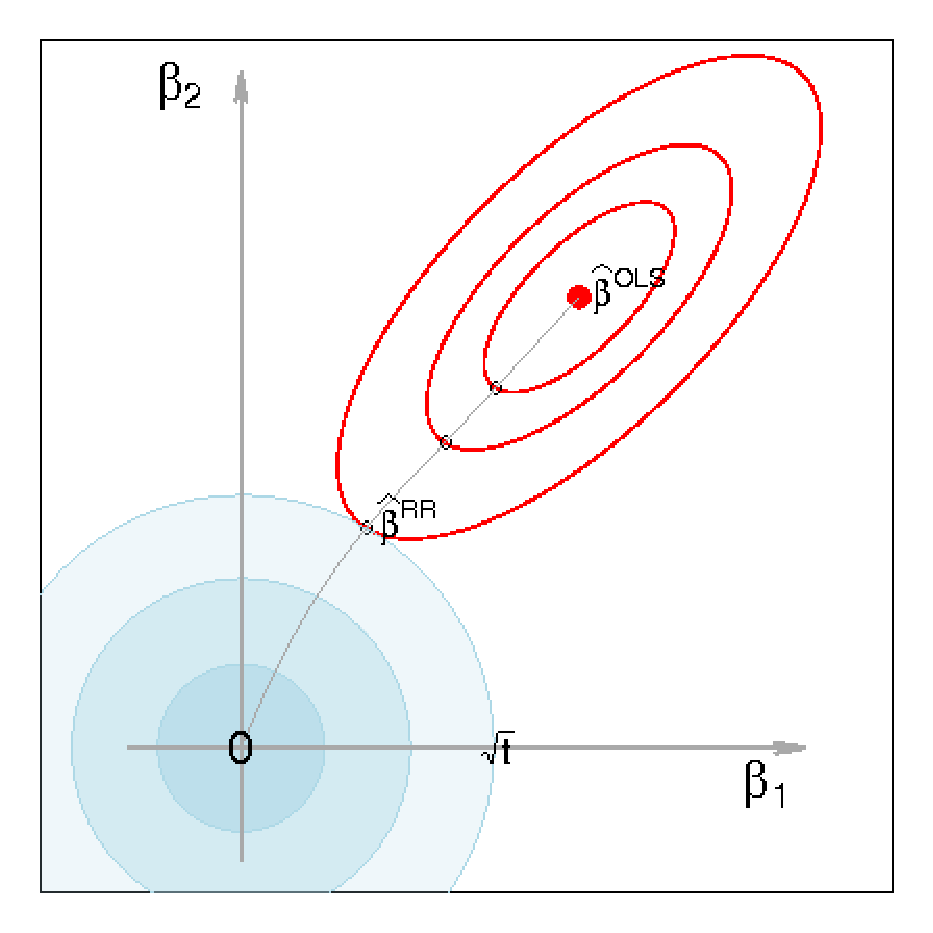
\includegraphics[width=.6\textwidth,clip]{fig/ridge-demo}
  \caption{Elliptical contours of the OLS residual sum of squares for two parameters in a regression, together with
  circular contours for the constraint function, $\beta_1^2 + \beta_2^2 \le t$. Ridge regression finds the point $\vec{\beta}^{RR}$ where
  the OLS contours just kiss the contstraint region.}%
  \label{fig:ridge-demo}
\end{figure}
The penalized Lagrangian formulation in \eqref{eq:ridgeRSS} has an equivalent form as a constrained
minimization problem,
\begin{equation}
\widehat{\vec{\beta}}^{\mathrm{RR}} = \argmin_{\vec{\beta}} (\vec{y}-\mat{X} \vec{\beta}) \trans  (\vec{y}-\mat{X} \vec{\beta})
  \quad\quad\mbox{subject to}\quad\quad
   \vec{\beta}\trans \vec{\beta} \le t(k)  \comma \label{eq:ridge}
\end{equation}
which makes the size constraint on the parameters explicit, with $t(k)$ an inverse function of $k$. This form provides
a visual interpretation of ridge regression, as shown in \figref{fig:ridge-demo}. Depicted in the figure are the
elliptical contours of the OLS regression sum of squares, $\mathrm{RSS}(0)$ around $\widehat{\vec{\beta}}^{\mathrm{OLS}}$.  Each
ellipsoid marks the point closest to the origin, i.e., with $\min \vec{\beta}\trans \vec{\beta}$.
It is easily seen that the ridge regression solution is the point where the elliptical contours just kiss the
constraint contour.

Another insightful interpretation of ridge regression \citep{Marquardt:1970} sees the ridge estimator as equivalent to
an OLS estimator, when the actual data in \mat{X} are supplemented by some number of fictitious observations, $n(k)$,
with uncorrelated predictors,
giving rise to
an orthogonal $\mat{X}_k^0$ matrix, and where $y=0$ for all supplementary observations. The linear model then becomes,

\begin{equation} \label{eq:ridge-sup1}
\left(
\begin{array}{c} \vec{y} \\ \vec{0} \end{array}
\right)
=
\left(
\begin{array}{c} \mat{X} \\ \mat{X}_k^0 \end{array}
\right)
\vec{\beta}^{\mathrm{RR}} \comma
\end{equation}
which gives rise to the solution,
\begin{equation} \label{eq:ridge-sup2}
\widehat{\vec{\beta}}^{\mathrm{RR}} = [\mat{X}\trans \mat{X} + (\mat{X}_k^0)\trans \mat{X}_k^0]^{-1} \mat{X}\trans \vec{y} \period
\end{equation}
But because $\mat{X}_k^0$ is orthogonal, $(\mat{X}_k^0)\trans \mat{X}_k^0$ is a scalar multiple of \mat{I}, so there
exists some value of $k$ making \eqref{eq:ridge-sup2} equivalent to \eqref{eq:ridge-beta}.  As promised, the
ridge regression estimator then reflects a weighted average of the data $[\mat{X}, \vec{y}]$ with $n(k)$ observations
$[\mat{X}_k^0, \vec{0}]$
biased toward $\vec{\beta}=\vec{0}$. In \figref{fig:ridge-demo}, it is easy to imagine that there is a direct translation between
the size of the constraint region, $t(k)$, and an equivalent supplementary sample size, $n(k)$, in this interpretation.

This classic version of the ridge regression problem can be generalized in a variety of ways, giving other geometric
insights.  Rather than a constant multiplier $k$ of \vec{\beta}\trans \vec{\beta} as the penalty term in \eqref{eq:ridgeRSS},
consider a penalty of the form $\vec{\beta}\trans \mat{K} \vec{\beta}$ with
a positive definite matrix \mat{K}.
The choice $\mat{K} = \diag (k_1, k_2, \dots)$ gives rise to a version of
\figref{fig:ridge-demo} in which the constraint contours are ellipses aligned with the coordinate axes, with
axis lengths inversely proportional to $k_i$.  These constants allow for differential shrinkage of the OLS coefficients.
The visual solution to the obvious modification of \eqref{eq:ridge} is again the point where the elliptical
contours of $\mathrm{RSS}(0)$ kiss the contours of the (now elliptical) constraint region.



